\documentclass[11pt]{article}
\usepackage[T1]{fontenc}
\usepackage{lmodern}
\usepackage[margin=1in]{geometry}
\usepackage{amsmath,amssymb}
\usepackage{graphicx}
\usepackage{booktabs}
\usepackage{xcolor}
\usepackage[numbers,sort&compress]{natbib}
\usepackage[hidelinks]{hyperref}
\usepackage{microtype}
\usepackage{eso-pic}
\usepackage{float}
\renewcommand{\topfraction}{0.95}\renewcommand{\bottomfraction}{0.9}
\renewcommand{\textfraction}{0.03}\renewcommand{\floatpagefraction}{0.85}
\setcounter{topnumber}{3}\setcounter{totalnumber}{4}
\usepackage[font=small,labelfont=bf,skip=4pt]{caption}

% Every measured number is a macro from paper/tables/numbers.tex
% (scripts/paper_numbers.py), so the text cannot drift from the data.
% AUTO-GENERATED by scripts/paper_numbers.py — do not edit by hand.
\newcommand{\dsBones}{247}
\newcommand{\dsSubjects}{12}
\newcommand{\dsTrain}{170}
\newcommand{\dsTrainSubj}{8}
\newcommand{\dsVal}{38}
\newcommand{\dsValSubj}{2}
\newcommand{\dsTest}{39}
\newcommand{\dsTestSubj}{2}
\newcommand{\dsPtsPerBone}{32{,}000}
\newcommand{\dsPtsTotalM}{7.9}
\newcommand{\dsCerv}{56}
\newcommand{\dsThor}{133}
\newcommand{\dsLumb}{55}
\newcommand{\dsLevels}{22}
\newcommand{\fracUnl}{46.0}
\newcommand{\fracSup}{9.2}
\newcommand{\fracInf}{9.1}
\newcommand{\fracPed}{4.5}
\newcommand{\fracBody}{23.5}
\newcommand{\fracSpin}{7.8}
\newcommand{\catClouds}{721}
\newcommand{\catProjects}{21}
\newcommand{\catModels}{26}
\newcommand{\catLabelFiles}{3{,}327}
\newcommand{\opsPointsM}{1}
\newcommand{\opsPickMs}{27}
\newcommand{\opsBoxMs}{29}
\newcommand{\opsLassoMs}{36}
\newcommand{\opsBrushMs}{9.2}
\newcommand{\opsApplyMs}{1.4}
\newcommand{\opsUndoMs}{0.6}
\newcommand{\opsRedoMs}{0.6}
\newcommand{\opsRepeats}{7}
\newcommand{\opsSlowestMs}{36}
\newcommand{\infMedianS}{2.4}
\newcommand{\infLoadS}{8}
\newcommand{\infWallS}{12}
\newcommand{\infBones}{6}
\newcommand{\infGpu}{RTX 4090}
\newcommand{\infPts}{32{,}000}
\newcommand{\valBones}{38}
\newcommand{\hiThresh}{0.99}
\newcommand{\sonSupPrec}{0.941}
\newcommand{\sonSupRec}{0.917}
\newcommand{\sonSupIou}{0.867}
\newcommand{\sonSupHi}{0.999}
\newcommand{\sonSupHiKept}{1532}
\newcommand{\sonSupWorst}{0.87}
\newcommand{\sonInfPrec}{0.920}
\newcommand{\sonInfRec}{0.928}
\newcommand{\sonInfIou}{0.859}
\newcommand{\sonInfHi}{0.996}
\newcommand{\sonInfHiKept}{1515}
\newcommand{\sonInfWorst}{0.78}
\newcommand{\sonPedPrec}{0.628}
\newcommand{\sonPedRec}{0.864}
\newcommand{\sonPedIou}{0.571}
\newcommand{\sonPedHi}{0.921}
\newcommand{\sonPedHiKept}{187}
\newcommand{\sonPedWorst}{0.30}
\newcommand{\sonMeanPrec}{0.830}
\newcommand{\sonMeanIou}{0.766}
\newcommand{\sonMeanHi}{0.972}
\newcommand{\sonMiouSix}{0.814}
\newcommand{\sonAxisS}{0.39}
\newcommand{\sonAxisSNinety}{2.4}
\newcommand{\sonAxisP}{1.5}
\newcommand{\sonAxisPNinety}{8.0}
\newcommand{\sonAxisC}{0.60}
\newcommand{\sonAxisCNinety}{1.4}
\newcommand{\sonAxisOk}{38}
\newcommand{\yamSupPrec}{0.934}
\newcommand{\yamSupRec}{0.910}
\newcommand{\yamSupIou}{0.855}
\newcommand{\yamSupHi}{0.987}
\newcommand{\yamSupHiKept}{1790}
\newcommand{\yamSupWorst}{0.84}
\newcommand{\yamInfPrec}{0.923}
\newcommand{\yamInfRec}{0.866}
\newcommand{\yamInfIou}{0.808}
\newcommand{\yamInfHi}{0.988}
\newcommand{\yamInfHiKept}{1605}
\newcommand{\yamInfWorst}{0.82}
\newcommand{\yamPedPrec}{0.638}
\newcommand{\yamPedRec}{0.858}
\newcommand{\yamPedIou}{0.577}
\newcommand{\yamPedHi}{0.833}
\newcommand{\yamPedHiKept}{555}
\newcommand{\yamPedWorst}{0.41}
\newcommand{\yamMeanPrec}{0.832}
\newcommand{\yamMeanIou}{0.747}
\newcommand{\yamMeanHi}{0.936}
\newcommand{\yamMiouSix}{0.804}
\newcommand{\yamAxisS}{0.63}
\newcommand{\yamAxisSNinety}{2.0}
\newcommand{\yamAxisP}{1.4}
\newcommand{\yamAxisPNinety}{6.3}
\newcommand{\yamAxisC}{1.00}
\newcommand{\yamAxisCNinety}{1.7}
\newcommand{\yamAxisOk}{38}
\newcommand{\dInfIou}{5.1}
\newcommand{\dSupIou}{1.2}
\newcommand{\dMiouSix}{0.9}


\newcommand{\lithium}{\textsc{Lithium}}
\newcommand{\gold}{Gold247}
\graphicspath{{figures/}}

% >>> arxiv-preview-stamp (make_arxiv.sh strips this block; arXiv adds its own)
\newcommand{\arxivid}{arXiv:2509.XXXXX v1\quad[cs.CV]\quad 29 Aug 2026}
\AddToShipoutPictureFG*{\AtPageLowerLeft{%
  \hspace{0.55cm}\raisebox{0.30\paperheight}{%
    \rotatebox{90}{\textcolor{gray!75}{\sffamily\footnotesize \arxivid}}}}}
% <<< arxiv-preview-stamp

\title{\vspace{-6mm}\lithium: a point-cloud annotation and in-loop training\\
  environment for anatomical surface labelling\vspace{-1mm}}
\author{Alexander Saffari\thanks{Correspondence: \texttt{alexwsaffari@gmail.com}.
  Code, data recipe and every figure script: \S\ref{sec:repro}.}}
\date{\today}

\begin{document}
\maketitle

\begin{abstract}
\noindent Anatomy is a surface. The landmarks that define a vertebra's coordinate
frame---endplates, pedicles, processes---lie on its outer surface, yet the tools
for labelling them work on volumes, slice by slice. \lithium{} labels anatomy as
surface point clouds instead: \dsPtsPerBone{} points per bone rather than
hundreds of thousands of voxels. It is a single desktop application in which the
catalog is the dataset, every stroke is persisted, Point Transformer models
\citep{wu2024ptv3,wu2025sonata} are trained in the loop, and the trained model
runs back on the next bone. Interaction stays inside one frame at
\opsPointsM{}\,M points (pick \opsPickMs{}\,ms, lasso \opsLassoMs{}\,ms). On
\gold{}---\dsBones{} hand-labelled VerSe vertebrae from \dsSubjects{}
subjects---two models trained inside the app reach endplate precision of
\sonSupPrec/\sonInfPrec{} on \valBones{} held-out bones, and the vertebral frame
derived from predicted labels agrees with the frame from hand labels to
\sonAxisS$^\circ$ (median). Pedicle precision (\sonPedPrec) is the open gap. The
annotation-timing study a tools paper owes is designed here and not yet run;
its slot is left visibly empty. \lithium{} is open source (MIT).
\end{abstract}

\noindent\textbf{Keywords:} point-cloud annotation; interactive segmentation;
vertebra; Point Transformer; in-the-loop training; open-source software

\begin{figure}[!htb]
  \centering
  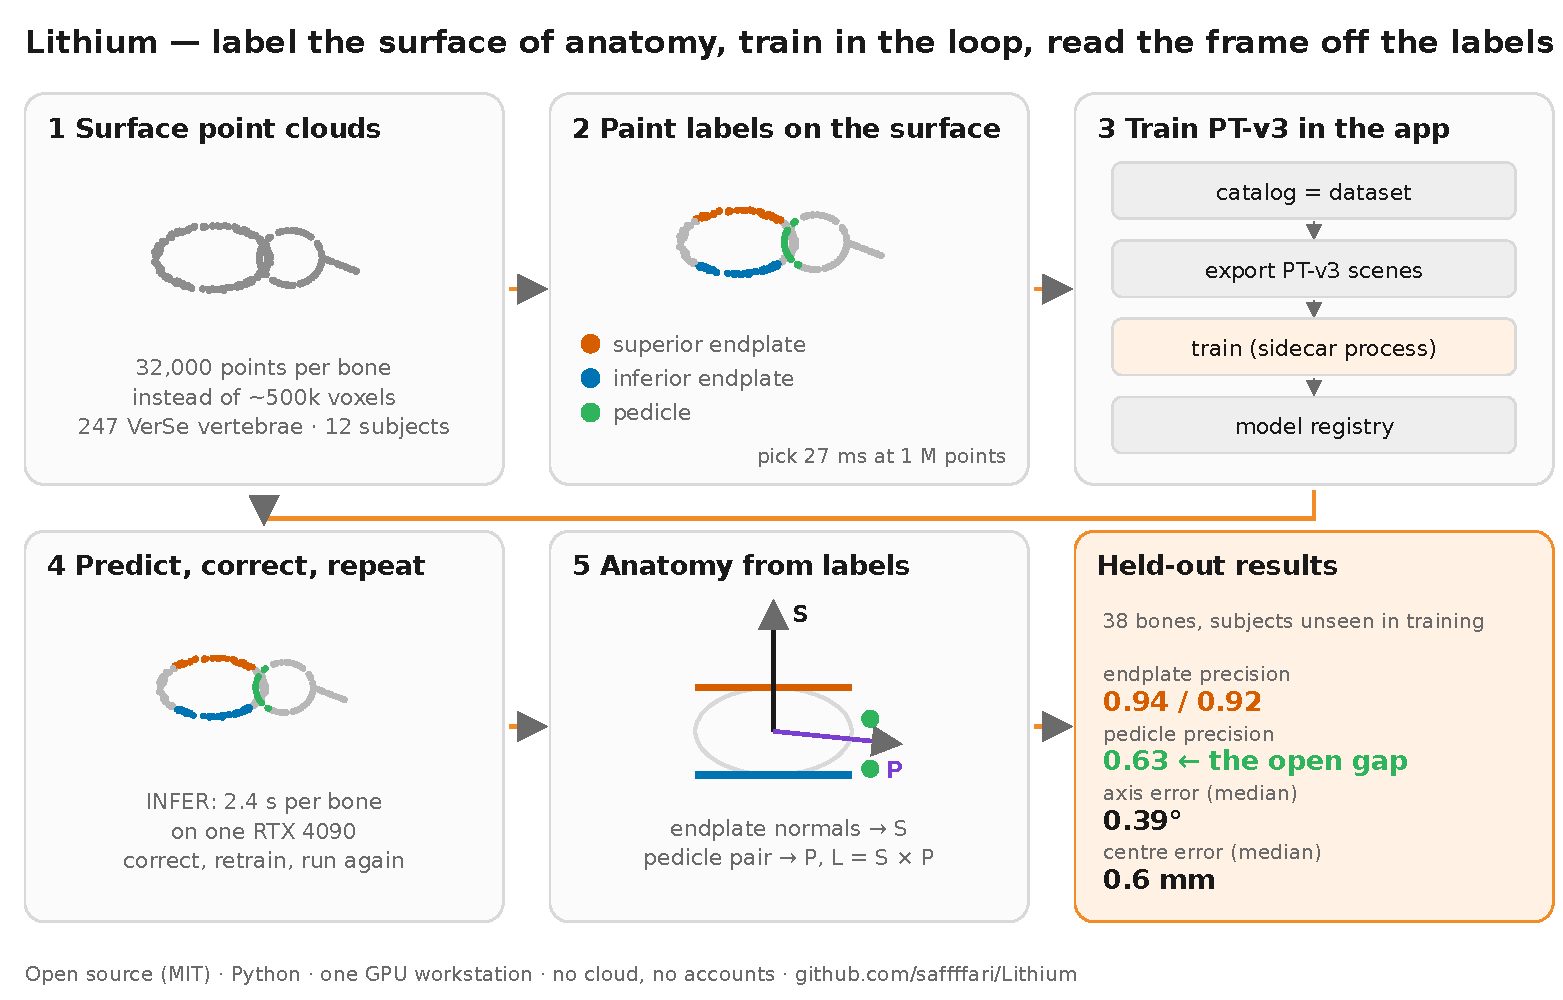
\includegraphics[width=0.92\textwidth]{fig_graphical_abstract}
  \caption{\textbf{Graphical abstract.} CT-derived vertebral surfaces are
  labelled as point clouds, the labels train a Point Transformer inside the
  app, the model predicts the next bone, and the local vertebral frame
  ($S$, $P$, $L$) is read directly off the labels. Numbers on the strip are the
  paper's headline results (\S\ref{sec:results}).}
  \label{fig:ga}
\end{figure}

\section{Why surfaces}
\label{sec:why}

Every voxel of a vertebra is bone; only its surface carries the anatomy that
measurements need. The superior and inferior endplates fix the cranio-caudal
axis, the pedicle pair fixes the posterior direction, and the two together give
a local frame \citep{stokes1994srs}. Volume labelling tools---3D~Slicer
\citep{fedorov2012slicer}, ITK-SNAP \citep{yushkevich2006itksnap}, and the
interactive learners built on top of them \citep{berg2019ilastik,isensee2025nninteractive}---make
the annotator paint through slices to reach that surface.
Figure~\ref{fig:concept} shows the alternative: extract the surface once
\citep{lorensen1987marching}, sample it to \dsPtsPerBone{} points, and label
\emph{those}. A bone's bounding box holds hundreds of thousands of 1\,mm$^3$
voxels; its surface needs \dsPtsPerBone{} points, and the labels on them are
sufficient to reconstruct the frame (Fig.~\ref{fig:concept}D--F).

Point-cloud annotation tools exist \citep{girardeau2016cloudcompare}, but none
close the loop: import, label, export, train, predict, correct---each step in a
different program. \lithium{} is that loop in one window
(Fig.~\ref{fig:ga}). Contributions:
\begin{itemize}\setlength\itemsep{1pt}
  \item a surface-first labelling environment whose catalog \emph{is} the
    dataset: content-hashed clouds, per-project ontologies and label
    namespaces, atomic persistence of every stroke, and a model registry with
    frozen class maps (\S\ref{sec:env}, Figs.~\ref{fig:env}--\ref{fig:datamodel});
  \item interaction that stays within a 60\,Hz frame at \opsPointsM{}\,M points
    and a one-click inference path that returns in seconds (Fig.~\ref{fig:latency});
  \item \gold{}: \dsBones{} VerSe vertebrae labelled with a six-class surface
    ontology, subject-split, with two models trained entirely inside the app and
    their errors traced to the anatomy (\S\ref{sec:results});
  \item a pre-registered timing protocol---two annotators, 30 bones, surface
    versus volume---whose results panel is deliberately left empty
    (\S\ref{sec:timing}).
\end{itemize}

\begin{figure}[!htb]
  \centering
  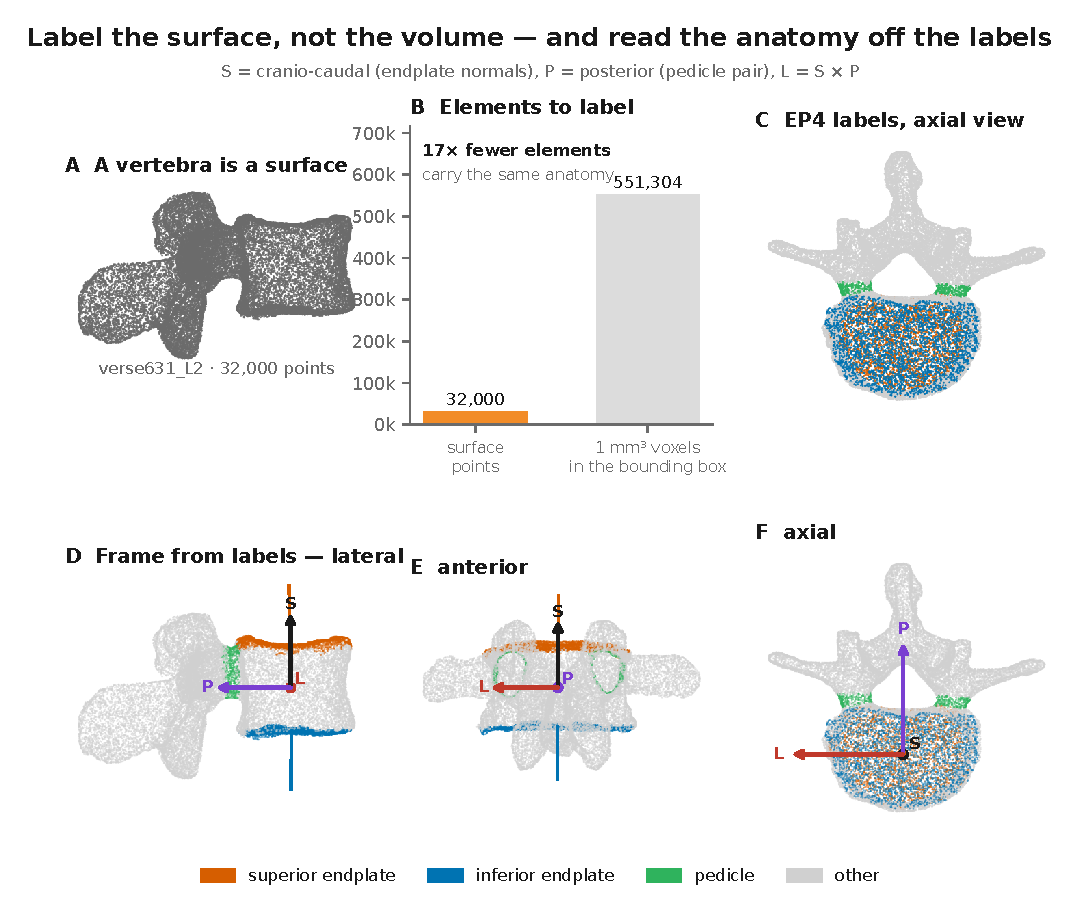
\includegraphics[width=\textwidth]{fig_concept}
  \caption{\textbf{Label the surface, not the volume.} (A)~A held-out \gold{}
  vertebra as a surface cloud. (B)~Elements an annotator must decide on:
  \dsPtsPerBone{} surface points versus the 1\,mm$^3$ voxels in the same bone's
  bounding box. (C)~The four-class EP4 ontology (superior endplate, inferior
  endplate, pedicle, other) on the axial view. (D--F)~The frame computed from
  those labels alone: endplate planes by SVD, $S$ from their normals, $P$ from
  the pedicle pair projected out of $S$, $L = S\times P$.}
  \label{fig:concept}
\end{figure}

\section{The environment}
\label{sec:env}

\paragraph{Three tabs, one loop.} \lithium{} is a Python desktop application
(ModernGL, GLFW, Dear ImGui \citep{cornut2024imgui}) organised as a pipeline
(Fig.~\ref{fig:env}). \textsc{Sheets} is the catalog: import PLY/LAS/NPZ clouds,
group them into projects, define each project's ontology, browse a gallery of
label-coloured previews. \textsc{Light Table} paints per-point labels with
pick, box, lasso, polygon, brush and curve tools, with undo for every
operation---including an applied prediction. \textsc{Train} stages a dataset
from the current labels, launches Pointcept \citep{pointcept2023} training in a
sidecar process, and registers the result. The registered model is then one
click away from any bone in the project.

\begin{figure}[!htb]
  \centering
  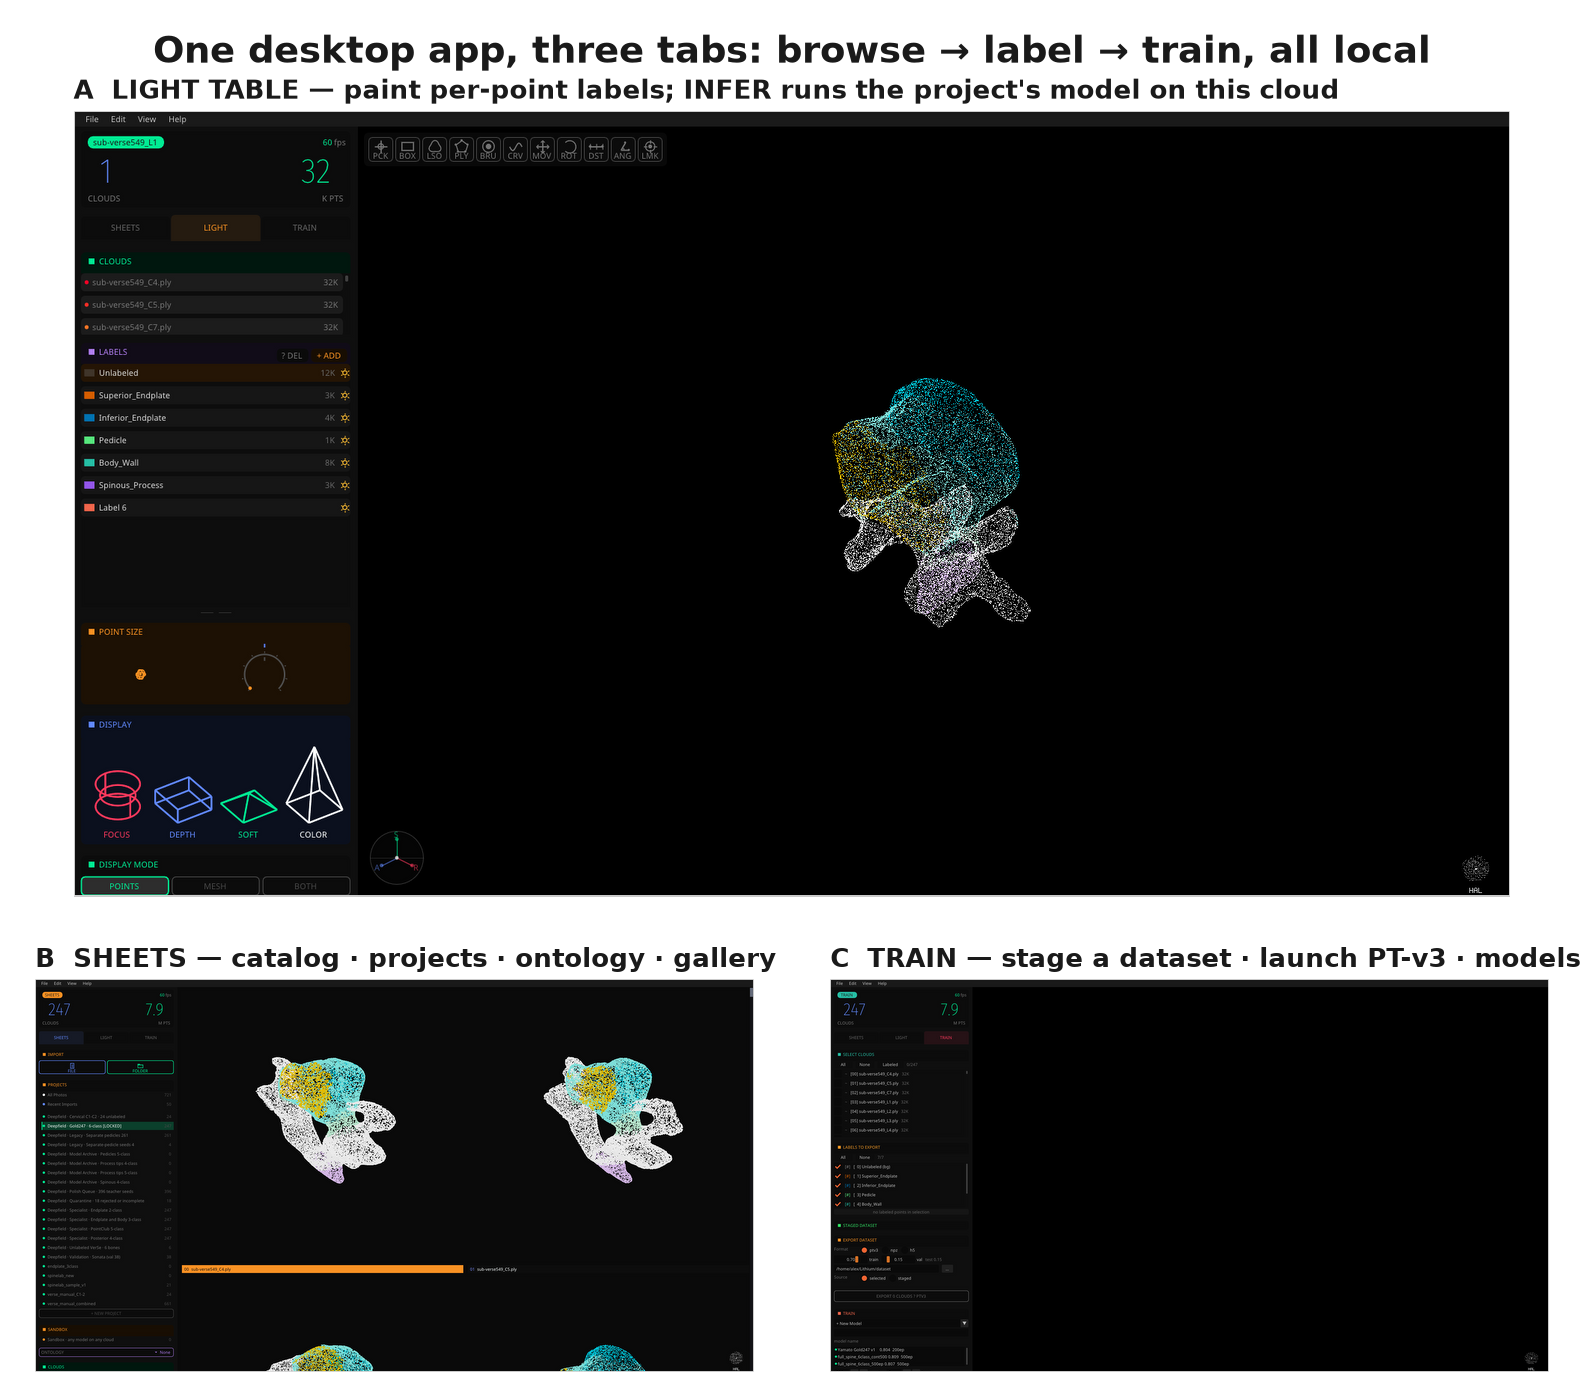
\includegraphics[width=\textwidth]{fig_environment}
  \caption{\textbf{The three tabs, on \gold{}.} (A)~\textsc{Light Table}: a
  hand-labelled L1 with the six-class ontology; the label list doubles as the
  paint palette. (B)~\textsc{Sheets}: projects in the left rail, label-coloured
  previews in the gallery. (C)~\textsc{Train}: cloud and class selection,
  dataset export, run launch and the model registry.}
  \label{fig:env}
\end{figure}

\paragraph{The catalog is the dataset.} Each imported cloud is content-hashed
and stored once; labels live in per-project namespaces, so the same bone can
carry a six-class ontology in one project and a two-class ontology in another
without either touching the other (Fig.~\ref{fig:datamodel}). Every stroke is
written atomically under the active namespace---there is no ``save project''
step and no way to lose labels by closing the window. A model's class map is
frozen at registration, so predictions are always interpreted against the
classes the network was trained on, not against whatever the ontology has
since become. A permanent \textsc{Sandbox} runs any registered model on any
cloud and stores the output as a cloud-level layer, so experimenting with a
model never pollutes a project's labels. The live catalog behind this paper
holds \catClouds{} clouds, \catProjects{} projects and \catModels{} registered
models.

\begin{figure}[!htb]
  \centering
  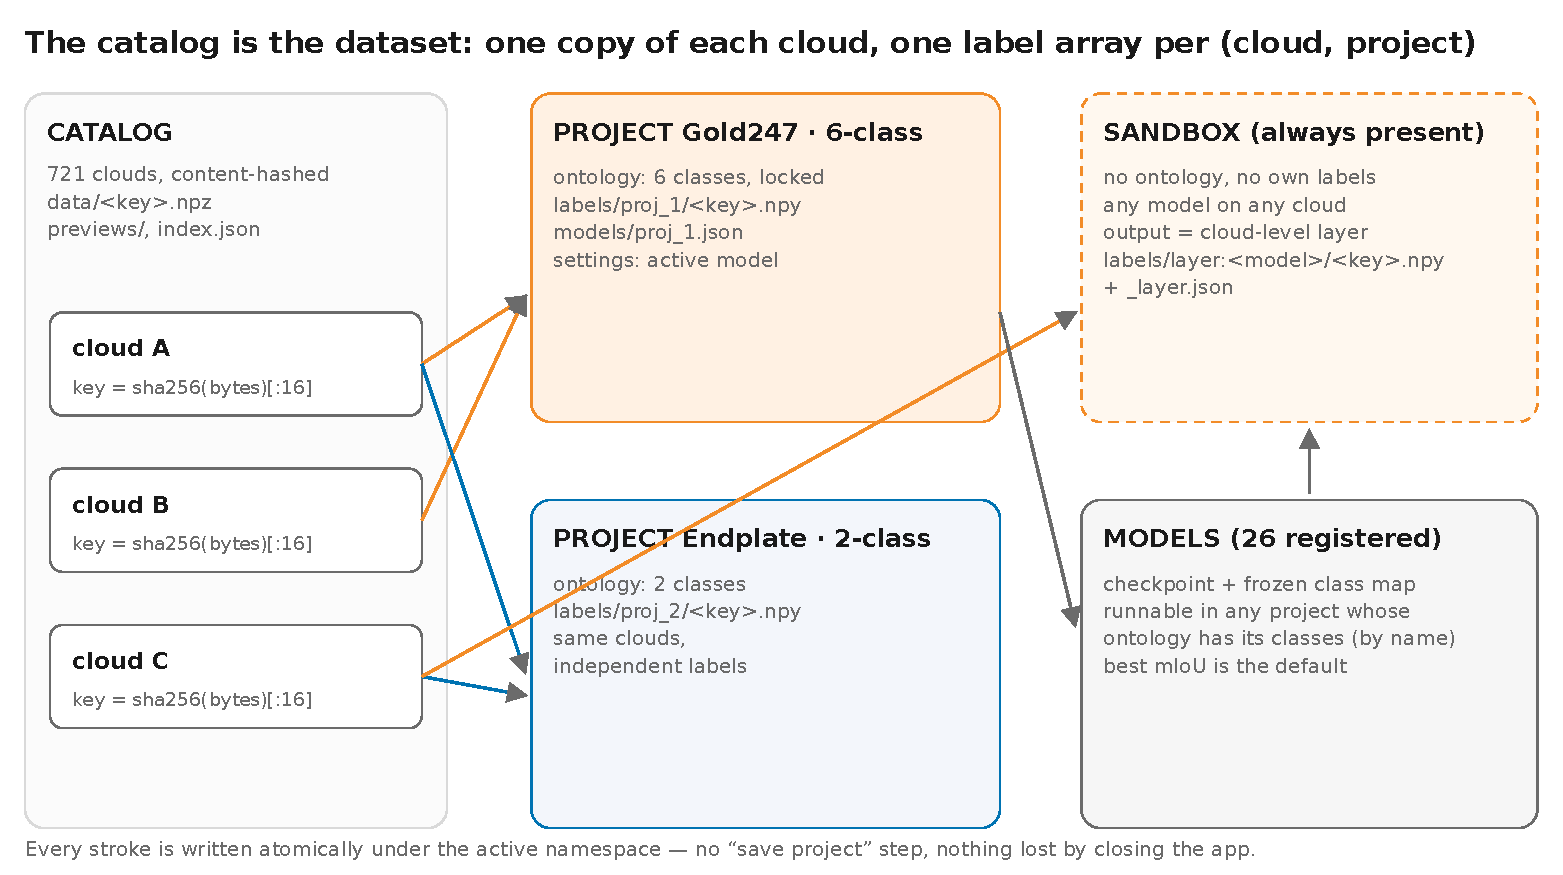
\includegraphics[width=\textwidth]{fig_data_model}
  \caption{\textbf{Data model.} One copy of each cloud; one label array per
  (cloud, project); projects own an ontology and a model registry; the sandbox
  owns nothing and writes cloud-level layers instead.}
  \label{fig:datamodel}
\end{figure}

\paragraph{Fast enough to forget.} Selection runs on the CPU over the full
cloud and uploads only the changed label bytes (Fig.~\ref{fig:latency}A):
at \opsPointsM{}\,M points a pick takes \opsPickMs{}\,ms, a lasso
\opsLassoMs{}\,ms, applying a label to half a million points \opsApplyMs{}\,ms
and undoing it \opsUndoMs{}\,ms (median of \opsRepeats{} runs). The slowest
operation, \opsSlowestMs{}\,ms, is still inside a couple of frames. Inference
is a subprocess call that reuses the training environment: on a
\infGpu{}, a \infPts{}-point bone is predicted in \infMedianS{}\,s once the
\infLoadS{}\,s model load is paid (Fig.~\ref{fig:latency}B).

\begin{figure}[!htb]
  \centering
  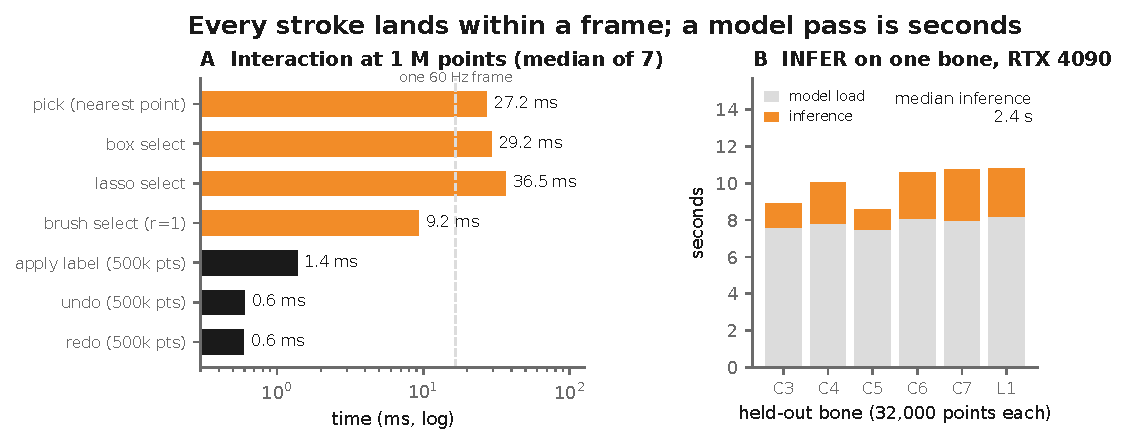
\includegraphics[width=\textwidth]{fig_latency}
  \caption{\textbf{Latency.} (A)~Selection and label operations on a synthetic
  \opsPointsM{}\,M-point cloud at $1920\times1080$, using the app's own code
  path; dashed line = one 60\,Hz frame. (B)~One-bone inference through the same
  script the \textsc{Infer} button spawns, \infBones{} held-out bones.}
  \label{fig:latency}
\end{figure}

\section{\gold{}}
\label{sec:data}

\gold{} is \dsBones{} vertebrae from \dsSubjects{} VerSe subjects
\citep{sekuboyina2021verse,loffler2020verse}, C3--L5, each a
\dsPtsPerBone{}-point surface sample of the reference segmentation, hand-labelled
in \lithium{} with six classes (Fig.~\ref{fig:dataset}). The split is by
subject---\dsTrain/\dsVal/\dsTest{} bones from \dsTrainSubj/\dsValSubj/\dsTestSubj{}
subjects---so no vertebra of a held-out patient is ever seen in training.
Endplates and pedicles together are \fracSup+\fracInf+\fracPed\,\% of the
points; they carry the frame, and they are what the models are scored on
(EP4: the six classes with body wall and spinous process folded into
``other'').

\begin{figure}[!htb]
  \centering
  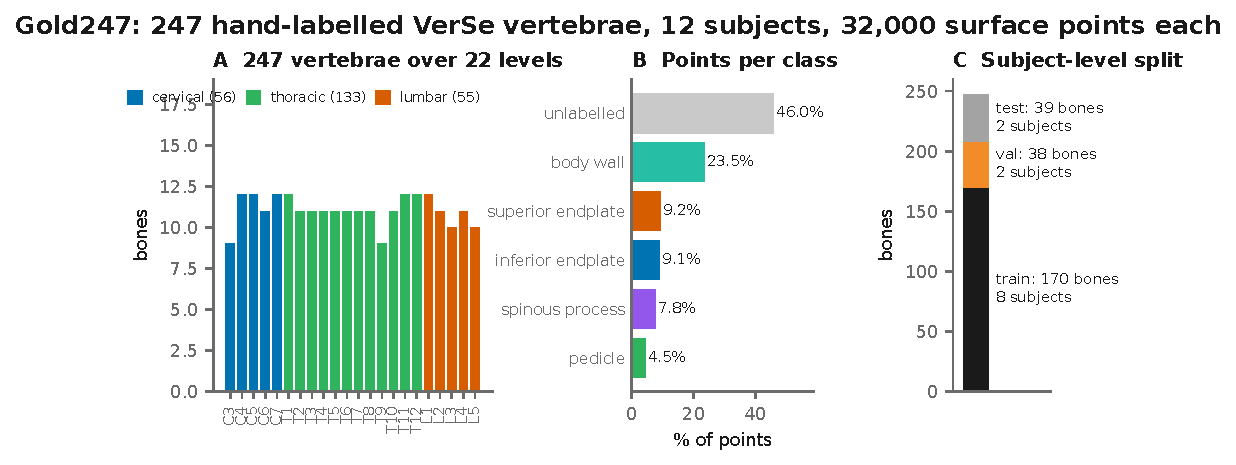
\includegraphics[width=\textwidth]{fig_dataset}
  \caption{\textbf{\gold{} at a glance.} (A)~Bones per level.
  (B)~Points per class over the whole set. (C)~Subject-level split.}
  \label{fig:dataset}
\end{figure}

\section{Results}
\label{sec:results}

Two models were trained inside the app on the same \dsTrain{} bones and scored
on the \valBones{} validation bones (Fig.~\ref{fig:results},
Table~\ref{tab:ep4}). \emph{Yamato} is Point Transformer~V3 \citep{wu2024ptv3}
from scratch; \emph{Sonata} is PT-v3m2 fine-tuned from the self-supervised
Sonata weights \citep{wu2025sonata}. Six-class validation mIoU is
\yamMiouSix{} and \sonMiouSix{} respectively.

\paragraph{Endplates are solved; pedicles are not.} Superior/inferior endplate
precision is \sonSupPrec/\sonInfPrec{} for Sonata (\yamSupPrec/\yamInfPrec{}
Yamato), with IoU up by \dSupIou{} and \dInfIou{} points. Pedicle precision is
\sonPedPrec{} versus \yamPedPrec{}---a tie, and the same failure in both:
predictions extend the pedicle label posteriorly along the arch into the
lamina (Fig.~\ref{fig:qual}). The error is a boundary convention, not noise; it
is the next labelling target, not the next architecture.

\paragraph{Confidence is honest.} Keeping only points the model assigns
$\geq\hiThresh$ confidence raises endplate precision to
\sonSupHi/\sonInfHi{} while retaining \sonSupHiKept/\sonInfHiKept{} points per
bone---enough for a plane fit---and pedicle precision to \sonPedHi{} on
\sonPedHiKept{} points (Fig.~\ref{fig:results}C).

\paragraph{The frame survives.} The local vertebral frame computed from
Sonata's labels deviates from the frame computed from hand labels by
\sonAxisS$^\circ$ in $S$ and \sonAxisP$^\circ$ in $P$ (medians;
\sonAxisSNinety$^\circ$ and \sonAxisPNinety$^\circ$ at the 90th percentile),
with the centre \sonAxisC{}\,mm off; Yamato gives \yamAxisS$^\circ$,
\yamAxisP$^\circ$ and \yamAxisC{}\,mm (Fig.~\ref{fig:results}E--G). Endplate
quality sets $S$; pedicle quality sets $P$.

\begin{figure}[!htb]
  \centering
  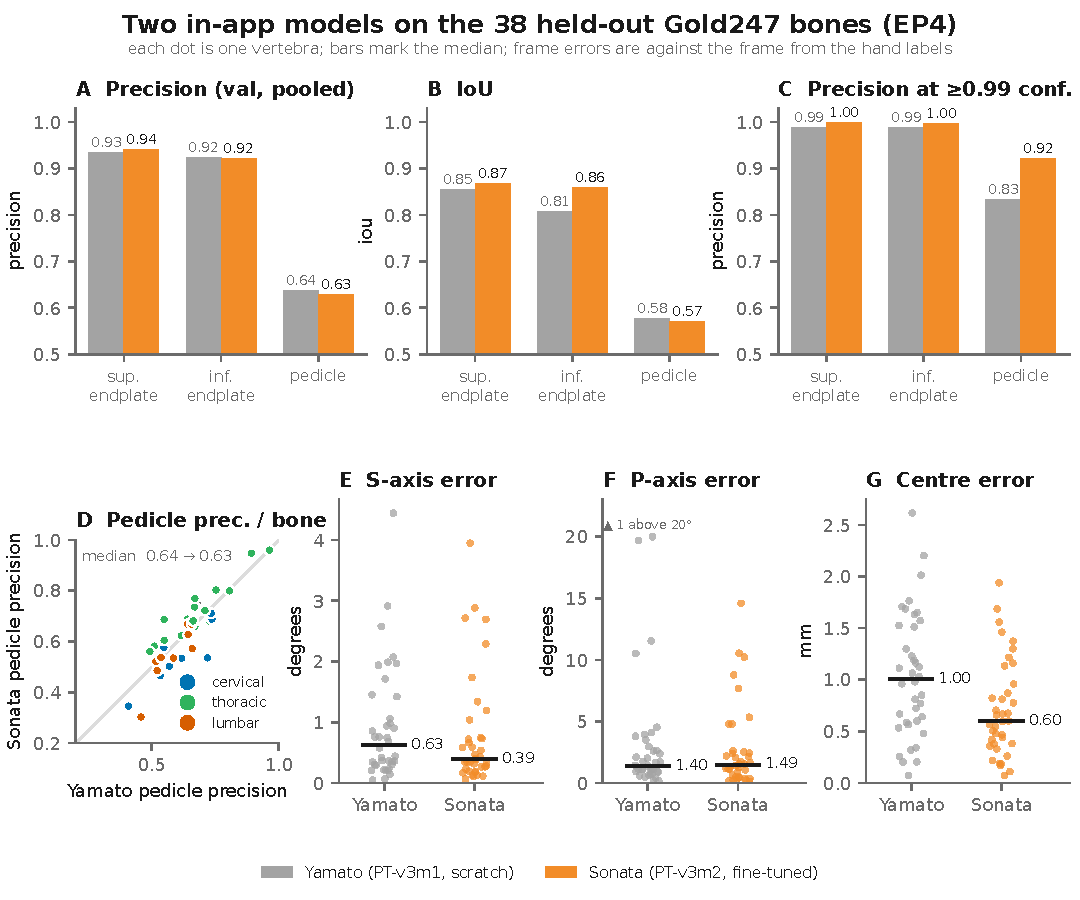
\includegraphics[width=\textwidth]{fig_results}
  \caption{\textbf{Two in-app models on the \valBones{} held-out bones.}
  (A--C)~Pooled precision, IoU and high-confidence precision per EP4 class.
  (D)~Per-bone pedicle precision, Yamato versus Sonata; colour = region.
  (E--G)~Errors of the frame derived from predicted labels against the frame
  from hand labels: cranio-caudal axis, posterior axis, centre.}
  \label{fig:results}
\end{figure}

\begin{table}[!htb]
  \centering\small
  \caption{EP4 results on the \valBones{} validation bones. Prec.\ / Rec.\ /
  IoU pooled over points; ``$\geq\hiThresh$'' = precision of points above that
  confidence and how many such points remain per bone.}
  \label{tab:ep4}
  \begin{tabular}{llcccrr}
    \toprule
    Model & Class & Prec. & Rec. & IoU & $\geq\hiThresh$ & kept/bone \\
    \midrule
    Yamato & sup.\ endplate & \yamSupPrec & \yamSupRec & \yamSupIou & \yamSupHi & \yamSupHiKept \\
           & inf.\ endplate & \yamInfPrec & \yamInfRec & \yamInfIou & \yamInfHi & \yamInfHiKept \\
           & pedicle        & \yamPedPrec & \yamPedRec & \yamPedIou & \yamPedHi & \yamPedHiKept \\
    \midrule
    Sonata & sup.\ endplate & \sonSupPrec & \sonSupRec & \sonSupIou & \sonSupHi & \sonSupHiKept \\
           & inf.\ endplate & \sonInfPrec & \sonInfRec & \sonInfIou & \sonInfHi & \sonInfHiKept \\
           & pedicle        & \sonPedPrec & \sonPedRec & \sonPedIou & \sonPedHi & \sonPedHiKept \\
    \bottomrule
  \end{tabular}
\end{table}

\begin{figure}[!htb]
  \centering
  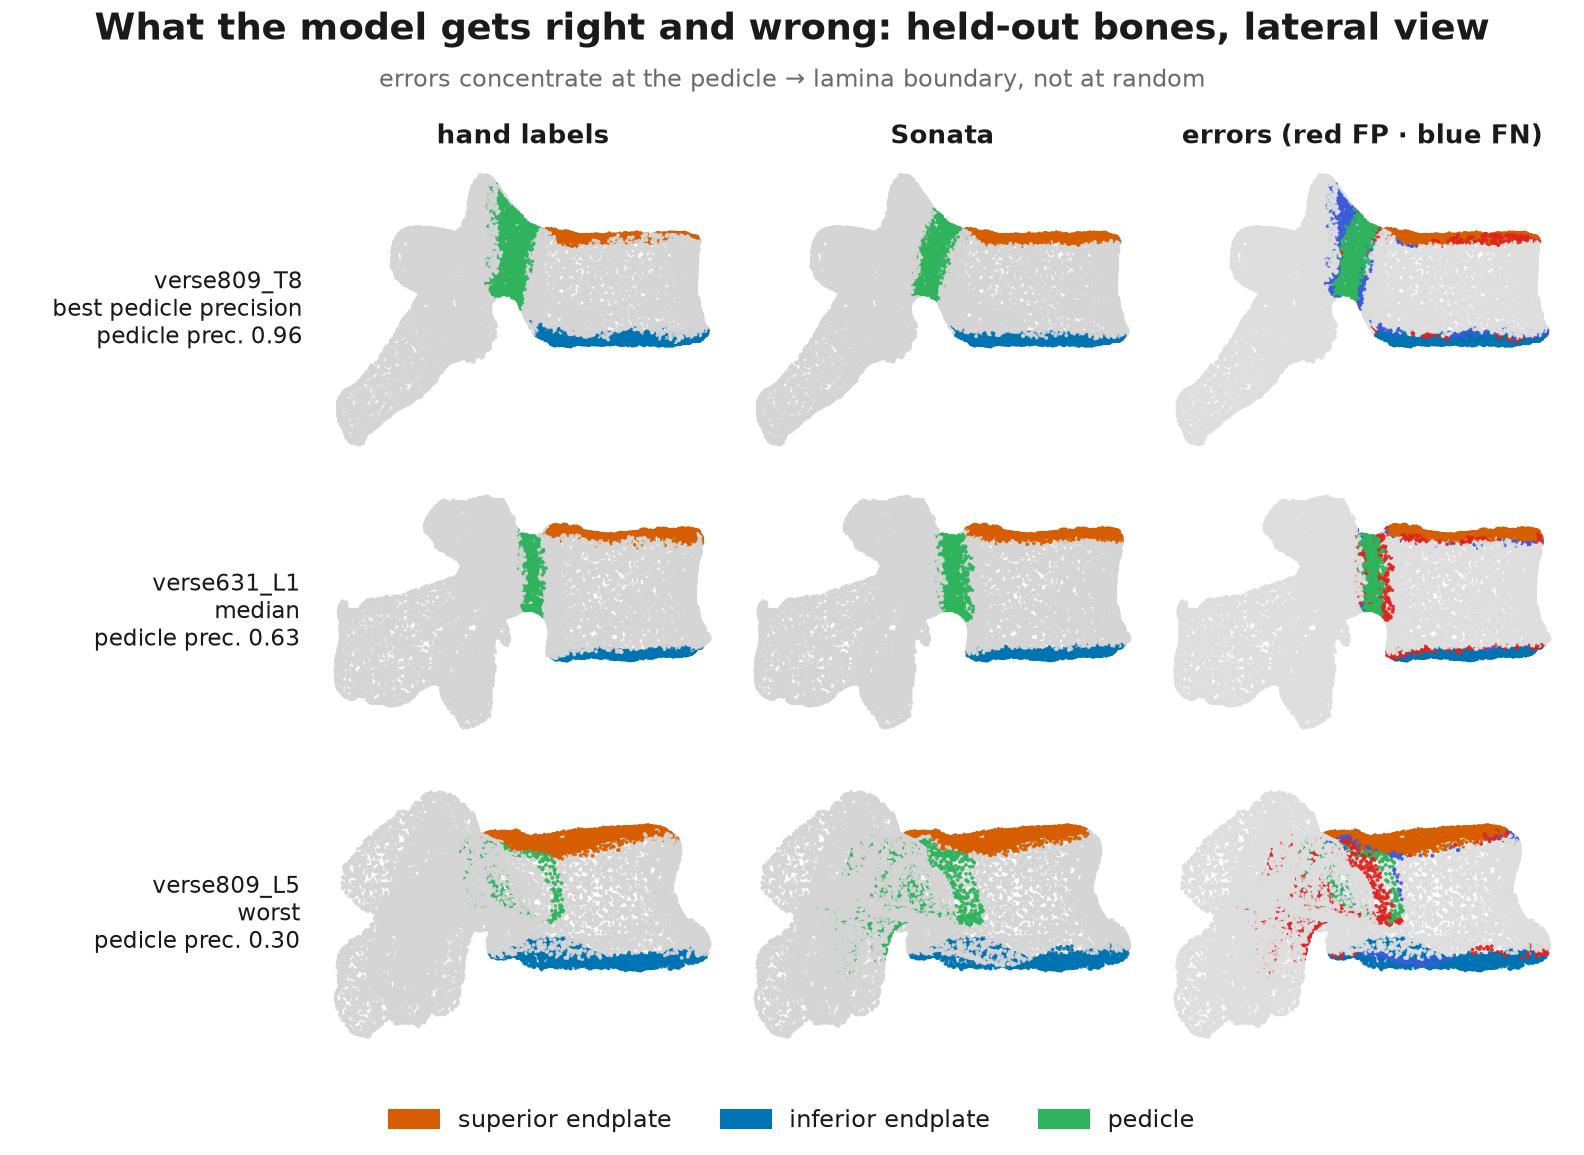
\includegraphics[width=0.92\textwidth]{fig_qualitative}
  \caption{\textbf{Where the errors are.} Best, median and worst held-out bones
  by pedicle precision: hand labels, Sonata's prediction, and the error map.
  Endplates are clean; the pedicle label leaks posteriorly into the lamina.}
  \label{fig:qual}
\end{figure}

\section{The timing study this paper owes}
\label{sec:timing}

The claim that motivates a surface-first tool---minutes per bone instead of
tens of minutes---has not been measured here. Figure~\ref{fig:timing} fixes the
protocol before the data exist: 30 bones from subjects unseen in \gold{}, ten
each cervical, thoracic and lumbar; two annotators, blind to each other; each
bone labelled once in \lithium{} (EP4 on the surface) and once by slice
painting in a volume tool; outcomes are minutes to completion, inter-annotator
point precision, and the frame error between the two annotators' labels. The
hypothesis is 3--5 versus 25--40 minutes per bone. Until the panels in
Fig.~\ref{fig:timing}B--C are filled, the throughput claim is a hypothesis and
is stated as one.

\begin{figure}[!htb]
  \centering
  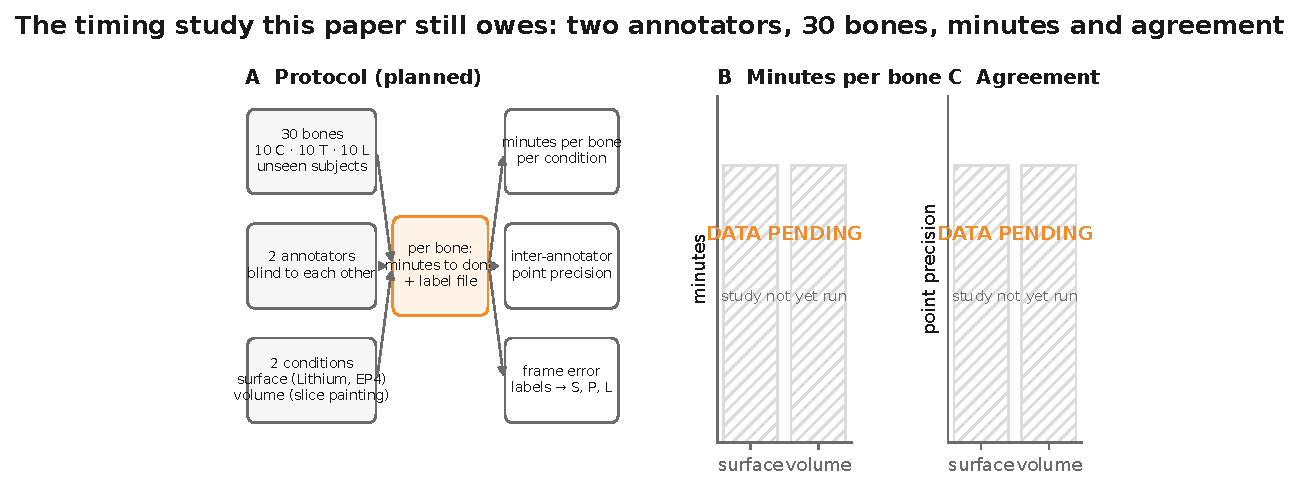
\includegraphics[width=\textwidth]{fig_timing_design}
  \caption{\textbf{Planned annotation-timing study.} (A)~Protocol.
  (B--C)~Result panels, intentionally empty: no timing data have been
  collected.}
  \label{fig:timing}
\end{figure}

\section{Limitations}

No timing or inter-annotator data yet (\S\ref{sec:timing}); \gold{} labels come
from a single labelling effort and their variability is unmeasured. Validation
is on \dsValSubj{} subjects (\valBones{} bones) of public VerSe data; patient
cohorts were used for qualitative checks only and appear nowhere in this
paper. Pedicle precision of \sonPedPrec{} is not yet sufficient for a
pedicle-driven posterior axis on every bone (worst bone \sonPedWorst). The
renderer needs OpenGL~4.3 and therefore does not run on macOS; a WebGPU
back-end is in progress. Rendering throughput at 1\,M+ points is not
instrumented and is described qualitatively.

\section{Availability and reproducibility}
\label{sec:repro}

{\sloppy
\lithium{} is MIT-licensed at \url{https://github.com/saffffari/Lithium}
(release v1.1). Every number in this paper is a LaTeX macro generated from a
result file: \texttt{scripts/paper\_dataset\_stats.py} (Fig.~\ref{fig:dataset}),
\texttt{paper\_bench\_ops.py} and \texttt{paper\_bench\_infer.py}
(Fig.~\ref{fig:latency}), \texttt{paper\_model\_metrics.py} (which re-scores
both models from their per-bone validation dumps; Fig.~\ref{fig:results},
Table~\ref{tab:ep4}) and \texttt{paper\_numbers.py}. Figures are rebuilt by
\texttt{paper\_figs.py}, \texttt{paper\_concept\_figs.py} and
\texttt{paper\_screenshots.py} (which drives the real application with
\texttt{--project/--cloud/--tab}). Only public VerSe-derived data are used; the
\gold{} export recipe and training configurations are in the repository.\par}

\section*{Acknowledgements}
\noindent [Placeholder: funding, data providers, colleagues --- to be filled by the author.]

\bibliographystyle{plainnat}
\bibliography{refs}
\end{document}
